\documentclass{standalone}
\begin{document}
% Interested in this interpretation of the Stab Rank as a quantifier of the resource
% Most obvious cross check seems to come from arbitrary states: access to the full state space through arbitrary rotations would be the ideal implementation of quantum computing
% However, Fault Tolerance necessitates that we are constrained in the set of operations and ancillae we use
% In the long run, resource choice will be blurred out
% But for small devices, the resource cost becomes signficant
% PBC outlined in the context of compiling a circuit for a device with a small number of qubits: seems like a huge reduction but really, 100 T-gates doesn't get you all that much!
% Different reource designs could impact how much computing power we get out of early quantum devices
%%%
% Face states: Asymptotic bound is larger, as is the strict lower bound
% Decompositions don't seem all that different but due to the initial slow divergence between the two scalings
% Include plot
% Big issue with the face state is it doesn't work in state injection
%%%
% Cn>3 states seem promising
% Could use simulated annealing to study them furhter
% DO work in state injection
%%%
% In any case, this work is just the beginning
% Any swich in resource state also needs to include circuit synthesis work to understand the saving better
As discussed in Section~\ref{sec:whybgss}, we are interested in understanding the stabiliser rank of a state as a potential quantifier of its value in quantum computation. This correspondence is predicated on the idea of using classical simulation to probe the quantum advantage, motivated by the Church-Turing-Deutsch thesis.\\
As noted by Jozsa \& Linden, however, the classical simulation complexity is strongly representation dependent. Assuming the validity of the thesis, the presence of an efficient classical simulation can be used to categorically rule out quantum speedup, but an inefficient classical description does not guarantee quantum advantage. Nonetheless, we argue that the stabiliser rank has the potential to constraint quantum speedup. Because it focuses on simulating universal quantum computations, we do not expect it to reduce to an efficient simulation. However, it does allow a relatively more efficient classical description of certain resource states, and thus it is interesting to probe the connection between $\chi$ and the value of different resources. 
\par
A simple confirmation of this concept large $T$-counts are required to implement quantum algorithms showing exponential speedup, described in Section~\ref{sec:whybgss}. Alternatively, we have shown in Table~\ref{tab:arbitrary} that these stabiliser decompositions offer little to no computational advantage for arbitrary quantum states; their stabiliser rank $\chi\approx2^{n}$. As previously mentioned, this can be understood as representing the ideal of `perfect' control of a quantum system. Access to arbitrary states suggests the ability to perform arbitrary single and multi-qubit operations with high-fidelity, as opposed to having to build them out of the elements of a universal gate set.\\
A reduction in stabiliser rank for resource states, and subsequently in the simulation complexity of the corresponding Clifford+`R' fault tolerant scheme, then has a natural correspondence to the increase in the number of elementary operations and physical qubits required to realise the same circuit relative to `perfect' control. 
\par
\section{Face-Type Magic States}
Under this interpretation, then, the proof presented in Section~\ref{sec:frank} would suggest that the face-type magic states serve as a stronger resource for quantum computation than the edge-type states, as they admit a smaller reduction in classical complexity. This is in fact congruent with the observation in~\cite{Howard2014} that the face-type states lead to a larger violation of contextuality inequalities than edge type states. This seems to further support the interpretation of contextuality as a resource for quantum computing. \\
The relative size of the scaling factors for the two families of magic states is given by
\begin{equation}
    \frac{\gamma_{F}}{\gamma_{H}} = \frac{\log_{2}\left(\cos(\beta)\right)}{\log_{2}\left(\cos(\frac{\pi}{8})\right)} = \frac{3}{2}
\end{equation}
which has a simple geometric interpretation in terms of the definition of each state: edge-type magic states are symmetric points between a pair of stabiliser states, whereas face-type states are the symmetric point between 3 stabiliser states. This can be seen in Fig.~\ref{fig:octahedron}. 
Interestingly, this ratio of $\frac{3}{2}$ is also the ratio of the \texttt{SL0} estimates of $\chi$ for single-copies of the $\ket{F}$ and $\ket{H}$ states. 
\par
However, despite the demonstration of a larger asymptotic bound, the explicit decompositions found for the two families of states were equal up to $4$ qubits. This is most likely a consequence of the small effect of the scaling factors for small number of qubits. The exponential scaling factors $2^{\gamma t}$ for each family of magic states are plotted in Fig.~\ref{fig:magicscale}. Here, you can see that the initial difference in the stabiliser rank is small, and that the two are approximately equal up to $5$ qubits. Thus, the lack of any apparent difference is a consequence of the computational constraints when finding these decompositions. 
\begin{figure}[t]
\centering
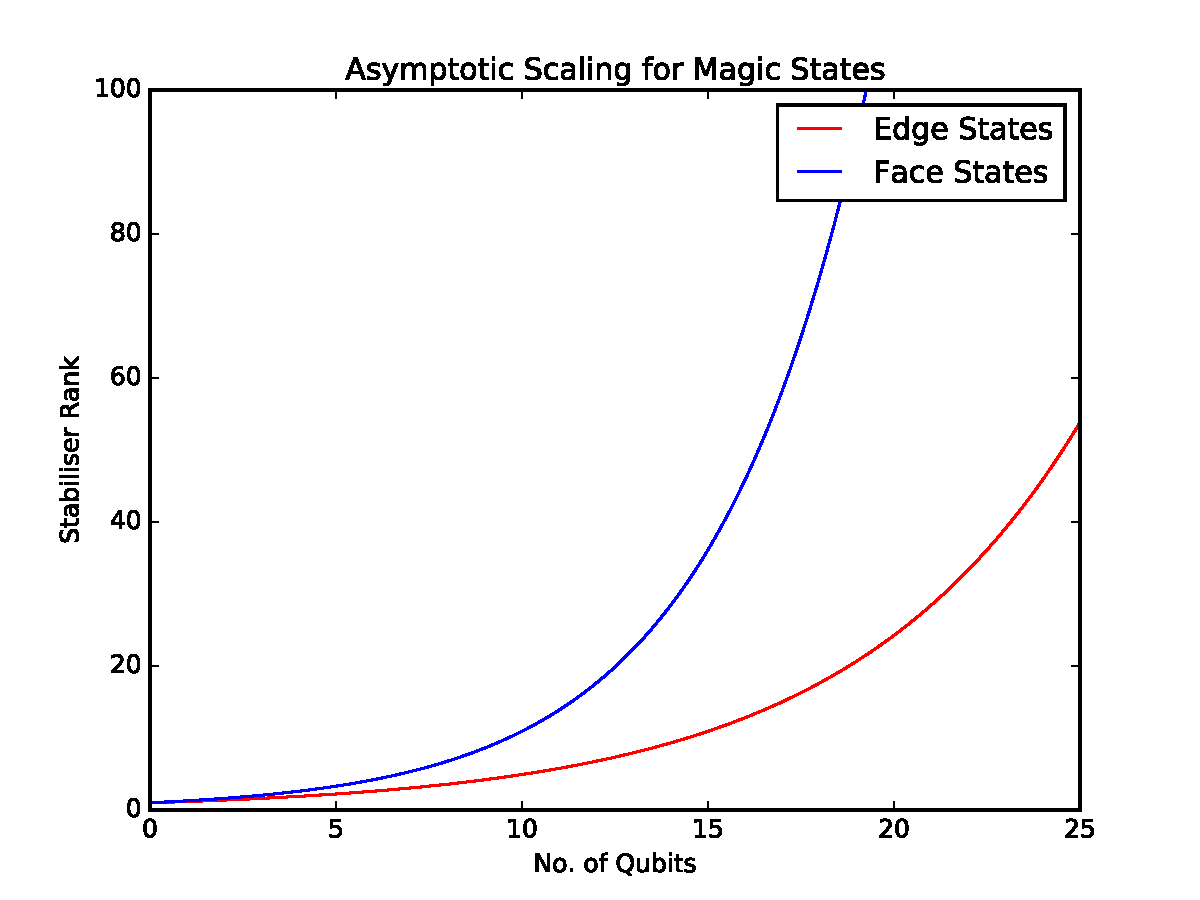
\includegraphics[width=0.75\textwidth]{Figures/magicrank.pdf}
\caption{Plot demonstrating the growth in the exponential scaling factors $2^{\gamma t}$ for both edge and face-type magic states.}
\label{fig:magicscale}
\end{figure}
\par
Unfortunately, a significant reason as to why the quantum computing community focus on the edge-type magic states is that there is currently no known circuit capable of using a face-type state to realise a gate from $\mathcal{C}_{3}$ \emph{deterministically}. The rotation $U:\ket{F}=U\ket{+}$ is equal to a $Y$-rotation followed by a $T$ gate. While demonstrably in $\mathcal{C}_{3}$ from Eq.~\ref{eq:resourcegate}, it is not a diagonal operator and thus the face-type states cannot be used in the state-injection circuit. In their original paper on magic state distillation, Bravyi \& Kitaev demonstrated a circuit that could, probabilistically, convert the state $\ket{F}\otimes\ket{F}$ to a resource state $\ket{A_{\frac{\pi}{6}}}$, that can be used to realise the gate $R_{\frac{\pi}{6}}$~\cite{Bravyi2005}, but no other circuit seems to exist in the literature. 

\section{$\mathcal{C}_{n>3}$ Resource States}
The resource states generated by taking successive roots of the $T$ gate, however, do satisfy the diagonality criteria, and thus can readily be consumed in a state injection circuit. This makes the increase in their stabiliser rank observed already at $2$ qubits especially interesting, as it would suggest that these states are immediately a better candidate resource than either family of magic state. \\
However, this is extrapolating these results from $2$ qubits, and so further research is needed to examine the stabiliser rank of these states. The \texttt{SL0} results seem to suggest a continued growth such that $\chi>\chi_{\text{magic}}$, but the power of this estimator is not well known. Given the seeming accuracy of Algorithm~\ref{alg:randwalk} up to $\ket{H^{\otimes 4}}$, this may serve as a better technique for studying the $\mathcal{C}_{n>3}$ states at higher $n$.

\section{Outlook for Quantum Computing}
As is clear form the case of arbitrary states, and from the lack of a known circuit for employing face-type magic states, a larger stabiliser rank does not immediately translate to a new, stronger resource for fault tolerant quantum computing. \\
There are several related questions that have to be considered when proposing a candidate resource for a Fault Tolerant scheme. Firstly, there is the question of consuming the resource; how readily can we employ it in our computation? 
\par
Secondly, we then have to consider the problem of preparing the resource fault tolerantly. For magic states, distillation schemes have been known and developed since 2005~\cite{Bravyi2005}. In particular, magic state distillation is based on performing stabiliser measurements on multiple, faulty copies, effectively performing quantum error correction to clean up errors in the preparation~\cite{Bravyi2005}. That this technique converges for magic states could perhaps be a direct consequence of their definition as symmetric points on the Bloch sphere between stabilisers.\\
Distillation schemes for alternative resource states are known. The most well developed alternative is Toffoli state distillation and injection, which was first developed by Shor in the earliest proposals on fault tolerant computing~\cite{Shor96}. In general, however, these Toffoli distillation schemes are slightly more resource intensive than magic state distillation~\cite{Eastin2013}. Most modern fault-tolerant proposals instead build a Toffoli gate in a circuit consuming $4-5$ magic states~\cite{Howard2016}. There seems to be a connection, then, between the computational power of the Toffoli gate (equivalent to several $T$ gates) and the resources required to distil the corresponding ancilla. This suggests that distillation schemes for alternative resource states likely exist, but that they may not be as efficient as magic state distillation. 
\par
The final question we have to consider is the problem of circuit synthesis: what are the resources required to implement a given computation in our chosen universal gate set? Current circuit synthesis techniques are best developed for the Clifford+T basis. There is known universal result, the Solovay-Kitaev theorem, for generating any arbitrary unitary in any gate set, but the resulting circuit complexity is known to be well in excess information theoretic bounds. Thus, the question of what resources different Clifford+R schemes require to implement a given computation remains open.\\
Come indications come from current fault-tolerant schemes, which require a certain number of $T$ gates to realise other unitary operations, such as the Toffoli example given above, but it is not yet known if these realisations are optimal. 
\par
When continued development in scalable qubit manufacturing and control allows us to build increasingly large quantum devices, these difference in resource costs will become less and less important; we will have sufficiently large physical resources that any universal construction will be realisable. However, in the near term, the resource costs represent a significant hurdle. \\
The PBC model of computing was derived by Bravyi, Smolin \& Smith in the context of trying to compile a quantum computation for implementation on a small quantum device with a fixed number of qubits, $O(10^{2})$. Initially, it might seem that the reduction of the circuit to a measurement on $t$ magic states represents a significant resource saving. But the rapid growth in the T-count of a circuit already discussed reveals the challenge of choosing a weak universal gate set. The seemingly minimal stabiliser rank of the edge-type magic states, and the existence of circuits requiring multiple $T$ gates to implement other useful $\mathcal{C}_{3}$ gates, does suggest that the Clifford+T basis is perhaps the most resource intensive choice for a universal fault tolerant design. Thus, the problem of developing alternative fault tolerant schemes becomes the problem of extracting as much computational power as possible from our early quantum devices. 
\ifstandalone
\bibliography{../MResProject.bib,../ManualEntries.bib}
\fi
\end{document}